\documentclass{article}
\usepackage{graphicx}
\usepackage{hyperref}
\usepackage{listings}
\usepackage{xcolor}
\usepackage{tikzsymbols}
\usepackage{float}

\lstset{
    basicstyle=\ttfamily,
    backgroundcolor=\color{gray!30},
}

\begin{document}

\graphicspath{ {./Images/} }
\tableofcontents

\section{Introduction}
It took me far too long to realize the significance of the word "Directory" in Active Directory.

\section{Domain Controller}

\subsection{Network}
To edit your network settings, follow these directions:

Control Panel $\rightarrow$ Network and Sharing Center $\rightarrow$
Change Adapter Settings $\rightarrow$ Click "Internet Protocol Version 4 (TCP/IPv4)

\begin{figure}[]
        \centering
        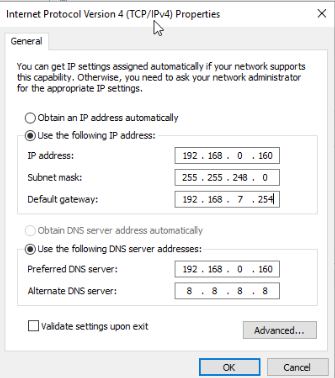
\includegraphics[width=1\textwidth]{SampleDCIPv4.png}
        \caption{Example IPv4 Settings}
        \label{fig:IPv4Settings}
\end{figure}

We have two goals in this menu: setting a static IP (to whatever) and setting the DNS servers. 
On non domain controllers, the DNS should be set to use DC1 and DC2.
On the domain controllers, the DNS should be set to use the other domain controller and the internet (e.g. 8.8.8.8 for Google's DNS).

\subsubsection{Setting a Static IP}
For an image, see Figure~\ref{fig:IPv4Settings}

You can set the static IP to any IP not currently in use.
(Maybe you can kick machines off of their IP, but that is probably not advised.)
Once you have picked your IP, put it in the \textbf{IP Address} field.
I am not sure how to determine the subnet mask manually, so I run \textbf{ipconfig} in powershell
and use the subnet mask it gives.
To determine the default gateway, you can run \textbf{ipconfig} or \textbf{route print}.
It is also possible to find the default gateway by running \textbf{ip route show} in the Proxmox console.


\subsubsection{Setting the DNS Servers}
For an image, see Figure~\ref{fig:IPv4Settings}

This step is less complicated than the last step. However, you can Red-Team yourself (I speak from experience...), so be careful.

On the Domain Controller, the first DNS server should be itself (the same as the machine's static IP). The second should be an actual internet DNS server.
In this case 8.8.8.8 is Google's DNS Server.

On non domain controllers, both DNS servers should point to the domain controllers.

\section{Useful Videos}
This is a list of useful videos for understanding active directory.
At some point I should watch all of the videos, take notes on them, and put them in the document.
\begin{enumerate}
        \item \href{https://youtu.be/n5suPvKqo_Y}{FSMO Roles} (not very good but idk what FSMO role are and it is important)
        \item \href{https://youtu.be/5rEA7vRV3VE}{Professor Messer LDAP/LDAPS}
        \item \href{https://youtu.be/2w1cesS7pGY}{Sean Metcalf Active Directory Overview}
        \item \href{https://youtu.be/ze1UcSLOypw}{Sean Metcalf Active Directory Attacks}
        \item \href{https://youtu.be/Lz6haohGAMc}{More Sean Metcalf Active Directory}
        \item\href{https://youtu.be/b6GUXerE9Ac}{Even more Sean Metcalf Active Directory}
        \item 
\end{enumerate}
\end{document}